\subsection{Applications}
\label{sec:application}


\begin{figure*}[t]
	\centering
	\subfloat[Scalability.\label{fig:kv_scalability}]
	{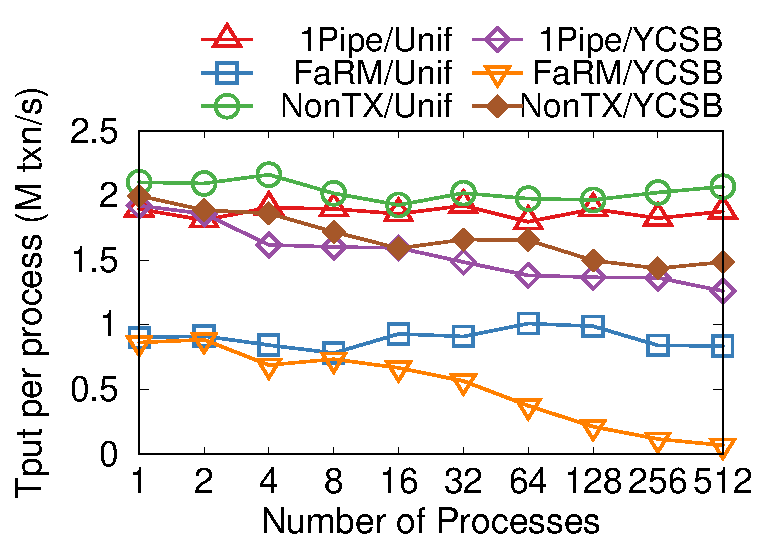
\includegraphics[width=.32\textwidth]{gnuplot/kv_scalability.eps}}
	\hspace{0.01\textwidth}
	\subfloat[Latency of YCSB workload.\label{fig:kv_latency_ycsb}]
	{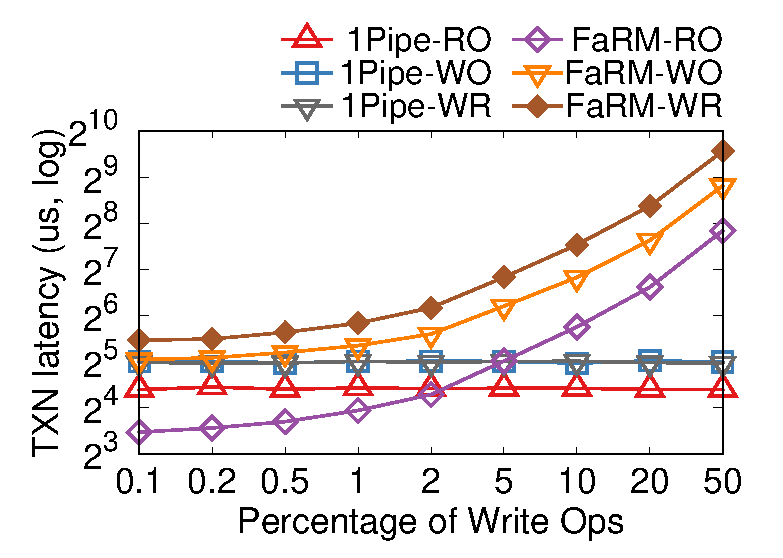
\includegraphics[width=.32\textwidth]{gnuplot/kv_latency_ycsb.eps}}
	\hspace{0.01\textwidth}
	\subfloat[Different transaction sizes.\label{fig:kv_multikey}]
	{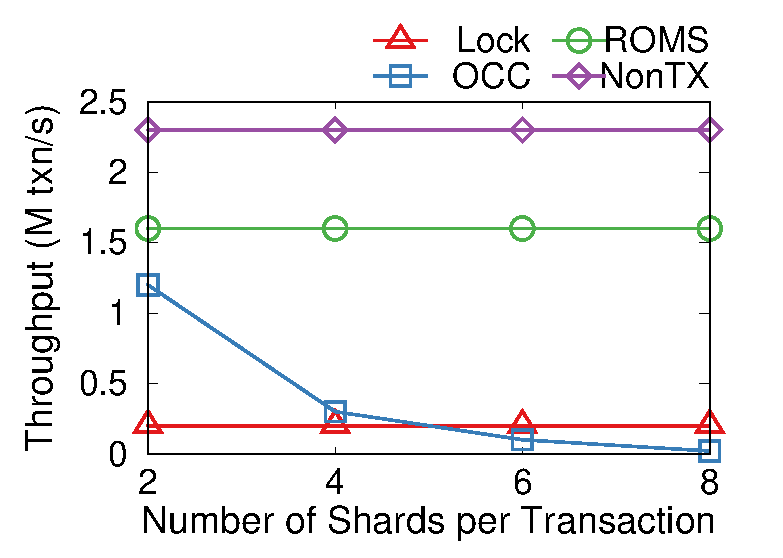
\includegraphics[width=.32\textwidth]{gnuplot/multishard.eps}}
	\vspace{-10pt}
	\caption{Performance of a transactional key-value store.}
	\vspace{-10pt}
\end{figure*}


\subsubsection{Transactional Key-Value Store}
\label{subsec:eval-kvs}


We evaluate a distributed transactional key-value store where each server process stores a portion of KVs in memory without replication using C++ \texttt{std::unordered\_map}.
A transaction (TXN) is composed of multiple independent KV read or write operations.
We use the same number of TXN initiator and server processes.
Initiator routes KV operations to servers by hash of key.
Read-only (RO) TXNs are served by best effort \sys{}, while read-write (WR) and write-only (WO) TXNs use reliable \sys{}.
For comparison, we implement non-replicated and non-durable FaRM~\cite{dragojevic2014farm} which serves RO TXNs in 1 RTT by reading the KVs and checking lock and version. WR and WO TXNs in FaRM use OCC~\cite{kung1981optimistic} and two-phase commit.
As a theoretical performance upper bound, we also compare with a non-transactional system.

Keys are 64-bit integers generated either uniformly random or by Zipf distribution in YCSB~\cite{cooper2010benchmarking}.
The value size is randomly generated according to Facebook's ETC workload~\cite{atikoglu2012workload}.
We record average TXN latency at 95\% of peak throughput.


In Figure~\ref{fig:kv_scalability}, we fix each TXN to have 2 KV ops, where read and write are randomly chosen for each op.


\textbf{Scalability of operations - Throughput - Number of processes - YCSB/Uniform. Expect: linear scale.}

In Figure~\ref{fig:kv_latency_ycsb}, We adjust the percentage of writes and measure TXN latency of RO, WO, and WR TXNs.

\sys{} is 90\% of NonTX. YCSB is 80\% of Uniform due to contention on hot keys. FaRM Uniform is 30\% of 1Pipe because each RW/RO TXN requires write, prepare, validate and commit steps. But FaRM YCSB is much worse because

\textbf{Comparison: NonTX, \sys{}, FaRM}

\textbf{Percentage of write ops - RO / WO / WR Latency (FaRM, 1Pipe) - YCSB. FaRM RO becomes higher with updates, because updated objects lead to TX aborts due to inconsistent version. WR also becomes higher due to high collision and abort rate (even higher than locking). Expect: in skewed workload, FaRM has higher transaction collision rate.}

When percentage of write ops is low - high success rate, base WO latency.

%\textbf{Write percentage - RO / WO / WR Latency - Uniform.}

%\textbf{Write percentage - Throughput - Uniform/YCSB. Expect: straight line vs. drop for high update percentage in FaRM (higher overhead). Not good, affect throughput due to different ops.}

FaRM RO latency = RTT / RO success rate
RO success rate = both objects are unlocked; value write version not broken.
FaRM WO latency = RTT * 3 (write, prepare + lock, commit + unlock) / WO success rate
WO success rate = write lock succeed.
FaRM WR latency = RTT * 4 (read/write, prepare + lock, validate, commit + unlock) / WO success rate
WR success rate = write lock succeed; read version correct.
\sys{} RO latency = RTT + best-effort reordering delay $\approx$ 2 RTT
\sys{} WR/WO latency = RTT + reliable reordering delay $\approx$ 3 RTT
NonTX latency = RTT

\sys{} / NonTX throughput: unchanged.
\sys{}  = NonTX / 1.1 due to additional round-trip in reliable.
FaRM throughput: NonTX / ((1/RO success rate + 1.4/WR success rate + 1.3/WO success rate) / 3).

50\% are read-only TXNs, 50\% are read-write TXNs.

In Figure~\ref{fig:kv_multikey}, 

\textbf{Number of KVs per TXN - Throughput - YCSB/Uniform. Expect: reverse proportional with number of objects, but NonTX and \sys{} are similar. More objects, higher contention rate.}



%\textbf{YCSB skewness - Throughput (50\% GET, 2 objects). Expect: in skewed workload, locking has higher transaction collision rate.}

%\textbf{YCSB skewness - Latency (50\% GET, 2 objects). Expect: slight increase in latency vs. high increase in latency due to aborts.}

%As a case study, we study the transaction performance of transactional key-value stores under YCSB+T~\cite{dey2014ycsbt} skewed workload.
%For the sake of simplicity, we focus on single round-trip (one-shot) transactions. Single-node transactions can be serialized on the server at the current timestamp, thus do not need \sys. General transactions with predetermined read and write sets can be reduced to single round-trip transactions, by sending the read and write set to each shard via \sys. During further execution of a general transaction, each shard can track the dependency and execute the read and write operations in timestamp order.

%Figure~\ref{fig:ycsb} shows the throughput and latency, where each atomic operation accesses two randomly chosen objects.
%\sys achieves 6.4~M transactions per server (0.8~M transactions per core) with 40~$\mu$s latency, close to an non-atomic system (NonTX) where operations are scattered directly without ordering.
%The throughput gap between \sys and NonTX is mainly due to CPU processing of reordering messages.
%The latency gap originates from the reordering delay.
%In comparison, the throughput of locks is limited by RTT.
%The throughput of centralized coordination is bottlenecked by the coordinator.

%Figure~\ref{fig:multishard} compares the single-core transaction throughput with an increasing number of keys per atomic scattering.
%Now we consider other timestamp-based methods.
%With more keys per scattering, the chance of transaction abort increases, because reordering in any one of the keys would cause transaction abort.

%Figure~\ref{fig:multishard} compares the throughput of TOMS, OCC, lock-based and non-transactional key-value stores.
%Each transaction accesses 8 unique remote objects.
%If the 8 objects are on two shards, OCC has 50\% chance of transaction abort, so the throughput is 50\% of non-transactional systems. When the objects are distributed on more shards, OCC has an exponentially higher chance of abort (Sec.~\ref{sec:toms}). The throughputs of other systems are unrelated to number of shards. \sys has 10x transaction throughput than lock-based systems, as well as OCC systems with more than 4 shards per transaction. The throughput of \sys is close to the theoretical bound of non-transactional system.

\iffalse
Finally, we study the efficiency of our loss detection and recovery mechanism in Sec.~\ref{sec:lossy}.
Assume 1/10 of the transactions have conflicts, \textit{i.e.}, if a transaction is rollbacked, 1/10 of uncommitted transactions also need rollback.
Figure~\ref{fig:ycsb-loss} simulates the transaction throughput and latency under different loss ratios.
With reliable \sys, packet loss is transparent to applications, and the transaction throughput is approximately the network goodput.
If \sys does not handle packet loss, the transaction processing application needs to rollback all uncommitted transactions on packet loss.

On the latency side, reliable \sys adds one RTT of latency to derive the delivery barrier.
If any packet is lost, reliable \sys needs to wait for an additional RTT to retransmit the packet.
When packet loss is rare, as in most data center networks, handling loss by applications provides lower latency.
Under high packet loss probability, however, handling losses in \sys is better.
\fi

\iffalse
\begin{figure}[t]
\centering

\includegraphics[width=0.3\textwidth]{images/fixme.pdf}
\caption{[Testbed] Comparing YCSB+T throughput on inter-DC WAN.}
\vspace{-10pt}
\label{fig:ycsb-inter-dc}
\end{figure}

Figure~\ref{fig:ycsb-inter-dc} compares the throughput of cross-datacenter workload of TOMS and lock-based.
\fi



\begin{figure*}[t]
	\centering
	\subfloat[New-Order 50\%, Payment 50\%.\label{fig:tpcc-combined}]
	{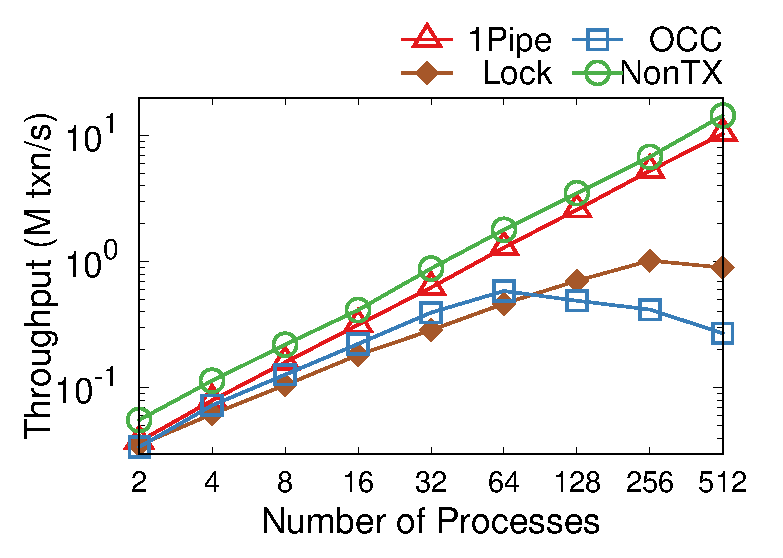
\includegraphics[width=.3\textwidth]{gnuplot/tpcc-combined.eps}}
	\hspace{0.02\textwidth}
	\subfloat[Payment 100\%.\label{fig:tpcc-payment}]
	{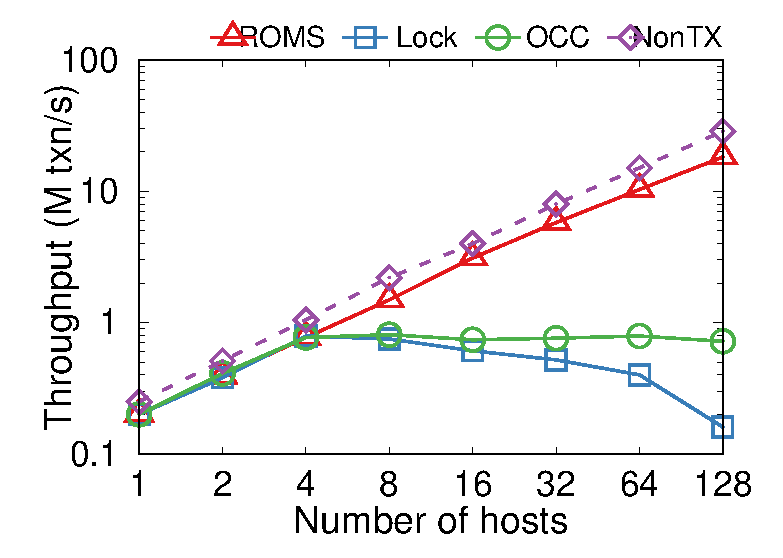
\includegraphics[width=.3\textwidth]{gnuplot/tpcc-payment.eps}}
	\hspace{0.02\textwidth}
	\subfloat[New-Order 100\%.\label{fig:tpcc-neworder}]
	{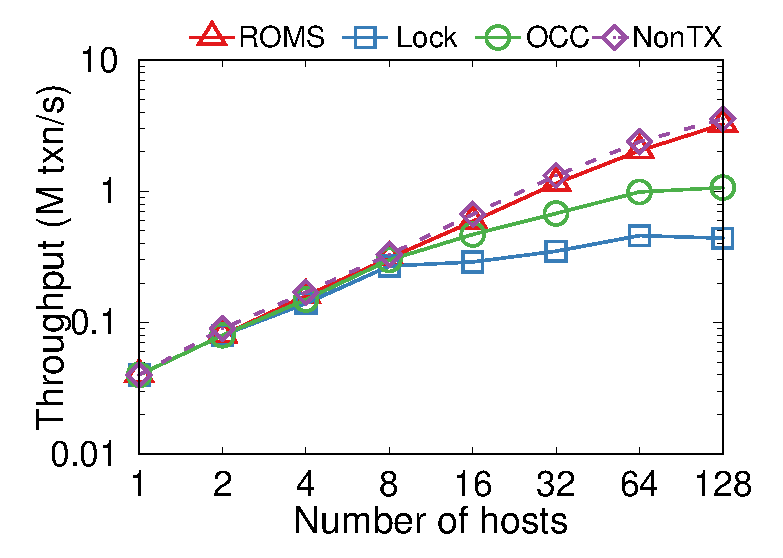
\includegraphics[width=.3\textwidth]{gnuplot/tpcc-neworder.eps}}
	\vspace{-10pt}
	\caption{TPC-C benchmark with 4 warehouses.}
	\label{fig:tpc-c}
	\vspace{-10pt}
\end{figure*}


\subsubsection{Independent General Transactions}
\label{subsec:eval-transactions}

We apply \sys to independent general transactions (Sec.\ref{subsec:dao}), which can be implemented with a batch of commands sent to all shards and replicas, similar to Eris~\cite{eris}.
We benchmark New-Order and Payment transactions in TPC-C~\cite{tpcc}, which constitute 90\% of TPC-C workload.
We assume the transactions never abort.
For simplicity, we do not implement non-independent transactions in TPC-C, which should fall back to traditional concurrency control mechanisms.
We use 4 warehouses which are stored in-memory with 3 replicas.
As shown in Figure~\ref{fig:tpc-c}, lock and OCC do not scale, because each Payment transaction updates its corresponding warehouse entry and each New-Order reads it~\cite{yu2014staring}.
The throughput of \sys scales linearly with number of concurrent hosts. With 128 hosts, \sys supports 18M Payment, 3.2M New-Order or 5.3M combined transactions, which is close to a non-transactional (NonTX) baseline system. With more hosts, the performance would be limited by CPU processing capacity of contended resources.

\textbf{Use one figure to save space.}

\subsubsection{Distributed Data Structures}
\label{subsec:data-structure}

Finally, we apply \sys{} to distributed data structures in order to remove ordering hazards (Sec.\ref{subsec:order-hazards}).
We implement a distributed concurrent hash table that uses a linked list to store key-value (KV) pairs in a same hash bucket, where hash buckets and KV pairs may be on different hosts.
Clients access the hash table using RDMA one-sided read, write and CAS atomics.
We measure KV insertion performance from one process on a host, while 16 processes on another host are looking up random keys.
Using \sys{}, KV insertion throughput improves from 311K to 590K (1.9x) operations per second.
This is because \sys{} removes the fence between writing KV pair and updating the pointer in hash bucket.
KV lookup throughput reduces from 325K to 312K op/s (4\% reduction), due to overhead in reordering delay.

If the hash table is replicated, a write op needs an additional RTT to the primary, which involves CPU software. However, reliable \sys{} does not need the client to wait for write completion.
With 3 replicas, \sys{} improves KV insertion throughput from 169K to 544K (3.2x) op/s.

\texttt{Failure recovery: faster than waiting for leader election triggered by raft heartbeat.}

We also apply \sys{} to Ceph~\cite{weil2006ceph} distributed storage. Ceph OSD uses a primary-backup replication scheme, where the backups are also written in order. With 3 replicas, a client waits for 3 disk writes and 6 network messages (3 RTTs) in sequence. With reliable \sys{}, the client can write 3 replicas in parallel, thus the end-to-end write latency is reduced to 1 disk write and 2 RTTs. Experimentation shows that in an idle system with Intel DC S3700 SSDs, 4KB random write average latency reduces from 160 $\mu$s to 58 $\mu$s (64\% reduction).


%\subsection{Multiple Round-Trip Transactions}

%TPC-C transaction benchmark

%Compare transaction throughput with Eris, TAPIR, DrTM+R (lock based), OCC and theoretical optimal (non-transactional)

%\subsection{Coordination-Free Causal Ordering}

%Our barrier timestamp is guaranteed to be lower than data timestamp, so if we send a message A after receiving a message B, A has higher timestamp than B. This can ensure ordering of events in a distributed system. For example, client A sends a command W to write database D, then sends a message to client B. When B receives the message from A, it sends command R to read database D. In our system, the database read command R is guaranteed to be processed after the write command W, so no additional synchronization is needed.